% Created by tikzDevice version 0.12.6 on 2024-01-08 11:43:12
% !TEX encoding = UTF-8 Unicode
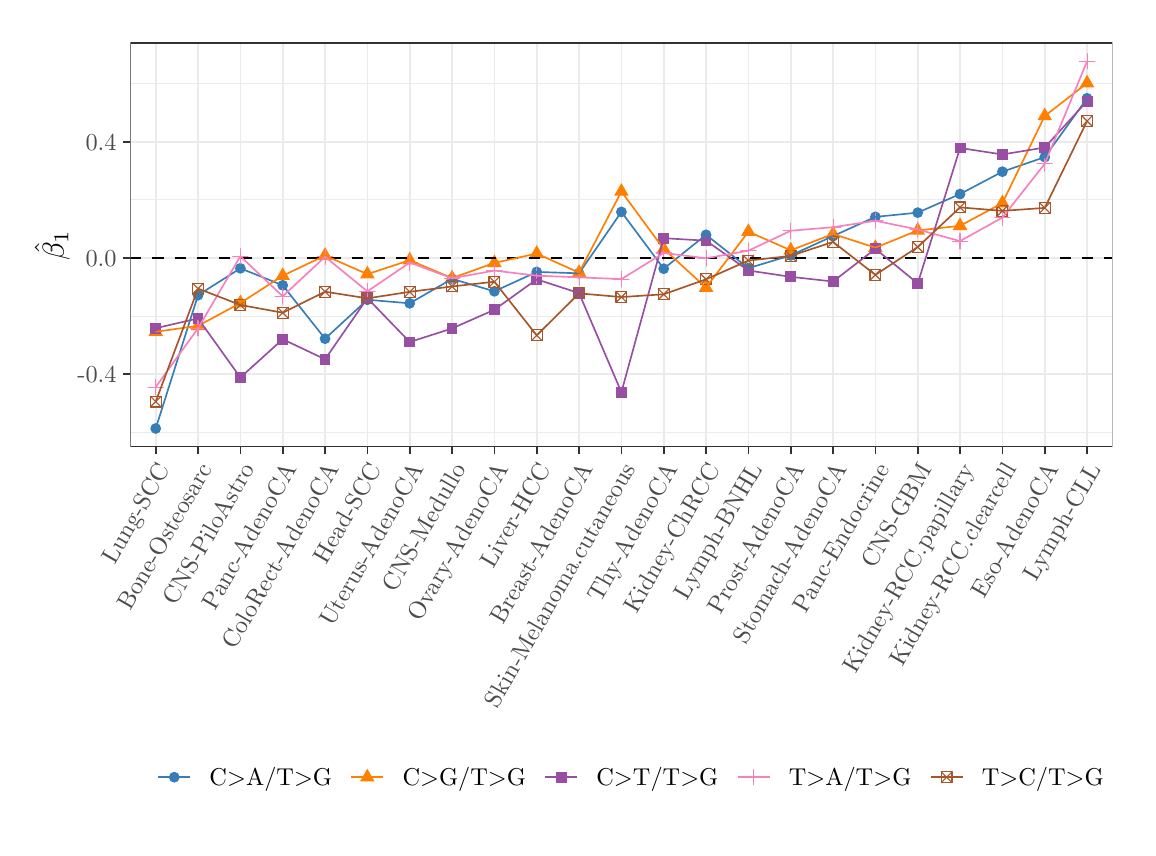
\begin{tikzpicture}[x=1pt,y=1pt]
\definecolor{fillColor}{RGB}{255,255,255}
\path[use as bounding box,fill=fillColor,fill opacity=0.00] (0,0) rectangle (397.48,289.08);
\begin{scope}
\path[clip] (  0.00,  0.00) rectangle (397.48,289.08);
\definecolor{drawColor}{RGB}{255,255,255}
\definecolor{fillColor}{RGB}{255,255,255}

\path[draw=drawColor,line width= 0.6pt,line join=round,line cap=round,fill=fillColor] (  0.00, -0.00) rectangle (397.48,289.08);
\end{scope}
\begin{scope}
\path[clip] ( 37.09,137.61) rectangle (391.98,283.58);
\definecolor{fillColor}{RGB}{255,255,255}

\path[fill=fillColor] ( 37.09,137.61) rectangle (391.98,283.58);
\definecolor{drawColor}{gray}{0.92}

\path[draw=drawColor,line width= 0.3pt,line join=round] ( 37.09,142.86) --
	(391.98,142.86);

\path[draw=drawColor,line width= 0.3pt,line join=round] ( 37.09,184.86) --
	(391.98,184.86);

\path[draw=drawColor,line width= 0.3pt,line join=round] ( 37.09,226.86) --
	(391.98,226.86);

\path[draw=drawColor,line width= 0.3pt,line join=round] ( 37.09,268.85) --
	(391.98,268.85);

\path[draw=drawColor,line width= 0.6pt,line join=round] ( 37.09,163.86) --
	(391.98,163.86);

\path[draw=drawColor,line width= 0.6pt,line join=round] ( 37.09,205.86) --
	(391.98,205.86);

\path[draw=drawColor,line width= 0.6pt,line join=round] ( 37.09,247.85) --
	(391.98,247.85);

\path[draw=drawColor,line width= 0.6pt,line join=round] ( 46.27,137.61) --
	( 46.27,283.58);

\path[draw=drawColor,line width= 0.6pt,line join=round] ( 61.56,137.61) --
	( 61.56,283.58);

\path[draw=drawColor,line width= 0.6pt,line join=round] ( 76.86,137.61) --
	( 76.86,283.58);

\path[draw=drawColor,line width= 0.6pt,line join=round] ( 92.16,137.61) --
	( 92.16,283.58);

\path[draw=drawColor,line width= 0.6pt,line join=round] (107.46,137.61) --
	(107.46,283.58);

\path[draw=drawColor,line width= 0.6pt,line join=round] (122.75,137.61) --
	(122.75,283.58);

\path[draw=drawColor,line width= 0.6pt,line join=round] (138.05,137.61) --
	(138.05,283.58);

\path[draw=drawColor,line width= 0.6pt,line join=round] (153.35,137.61) --
	(153.35,283.58);

\path[draw=drawColor,line width= 0.6pt,line join=round] (168.65,137.61) --
	(168.65,283.58);

\path[draw=drawColor,line width= 0.6pt,line join=round] (183.94,137.61) --
	(183.94,283.58);

\path[draw=drawColor,line width= 0.6pt,line join=round] (199.24,137.61) --
	(199.24,283.58);

\path[draw=drawColor,line width= 0.6pt,line join=round] (214.54,137.61) --
	(214.54,283.58);

\path[draw=drawColor,line width= 0.6pt,line join=round] (229.83,137.61) --
	(229.83,283.58);

\path[draw=drawColor,line width= 0.6pt,line join=round] (245.13,137.61) --
	(245.13,283.58);

\path[draw=drawColor,line width= 0.6pt,line join=round] (260.43,137.61) --
	(260.43,283.58);

\path[draw=drawColor,line width= 0.6pt,line join=round] (275.73,137.61) --
	(275.73,283.58);

\path[draw=drawColor,line width= 0.6pt,line join=round] (291.02,137.61) --
	(291.02,283.58);

\path[draw=drawColor,line width= 0.6pt,line join=round] (306.32,137.61) --
	(306.32,283.58);

\path[draw=drawColor,line width= 0.6pt,line join=round] (321.62,137.61) --
	(321.62,283.58);

\path[draw=drawColor,line width= 0.6pt,line join=round] (336.91,137.61) --
	(336.91,283.58);

\path[draw=drawColor,line width= 0.6pt,line join=round] (352.21,137.61) --
	(352.21,283.58);

\path[draw=drawColor,line width= 0.6pt,line join=round] (367.51,137.61) --
	(367.51,283.58);

\path[draw=drawColor,line width= 0.6pt,line join=round] (382.81,137.61) --
	(382.81,283.58);
\definecolor{fillColor}{RGB}{55,126,184}

\path[fill=fillColor] ( 61.56,192.41) circle (  1.96);
\definecolor{fillColor}{RGB}{255,127,0}

\path[fill=fillColor] ( 61.56,184.37) --
	( 64.21,179.79) --
	( 58.92,179.79) --
	cycle;
\definecolor{fillColor}{RGB}{152,78,163}

\path[fill=fillColor] ( 59.60,182.06) --
	( 63.53,182.06) --
	( 63.53,185.99) --
	( 59.60,185.99) --
	cycle;
\definecolor{drawColor}{RGB}{247,129,191}

\path[draw=drawColor,line width= 0.4pt,line join=round,line cap=round] ( 58.79,180.46) -- ( 64.34,180.46);

\path[draw=drawColor,line width= 0.4pt,line join=round,line cap=round] ( 61.56,177.69) -- ( 61.56,183.24);
\definecolor{drawColor}{RGB}{166,86,40}

\path[draw=drawColor,line width= 0.4pt,line join=round,line cap=round] ( 59.60,192.83) rectangle ( 63.53,196.76);

\path[draw=drawColor,line width= 0.4pt,line join=round,line cap=round] ( 59.60,192.83) -- ( 63.53,196.76);

\path[draw=drawColor,line width= 0.4pt,line join=round,line cap=round] ( 59.60,196.76) -- ( 63.53,192.83);
\definecolor{fillColor}{RGB}{55,126,184}

\path[fill=fillColor] (199.24,200.32) circle (  1.96);
\definecolor{fillColor}{RGB}{255,127,0}

\path[fill=fillColor] (199.24,203.59) --
	(201.88,199.01) --
	(196.60,199.01) --
	cycle;
\definecolor{fillColor}{RGB}{152,78,163}

\path[fill=fillColor] (197.28,191.20) --
	(201.20,191.20) --
	(201.20,195.12) --
	(197.28,195.12) --
	cycle;
\definecolor{drawColor}{RGB}{247,129,191}

\path[draw=drawColor,line width= 0.4pt,line join=round,line cap=round] (196.46,198.85) -- (202.01,198.85);

\path[draw=drawColor,line width= 0.4pt,line join=round,line cap=round] (199.24,196.07) -- (199.24,201.62);
\definecolor{drawColor}{RGB}{166,86,40}

\path[draw=drawColor,line width= 0.4pt,line join=round,line cap=round] (197.28,191.11) rectangle (201.20,195.03);

\path[draw=drawColor,line width= 0.4pt,line join=round,line cap=round] (197.28,191.11) -- (201.20,195.03);

\path[draw=drawColor,line width= 0.4pt,line join=round,line cap=round] (197.28,195.03) -- (201.20,191.11);
\definecolor{fillColor}{RGB}{55,126,184}

\path[fill=fillColor] (321.62,222.24) circle (  1.96);
\definecolor{fillColor}{RGB}{255,127,0}

\path[fill=fillColor] (321.62,218.84) --
	(324.26,214.27) --
	(318.98,214.27) --
	cycle;
\definecolor{fillColor}{RGB}{152,78,163}

\path[fill=fillColor] (319.66,194.70) --
	(323.58,194.70) --
	(323.58,198.63) --
	(319.66,198.63) --
	cycle;
\definecolor{drawColor}{RGB}{247,129,191}

\path[draw=drawColor,line width= 0.4pt,line join=round,line cap=round] (318.84,216.15) -- (324.39,216.15);

\path[draw=drawColor,line width= 0.4pt,line join=round,line cap=round] (321.62,213.38) -- (321.62,218.93);
\definecolor{drawColor}{RGB}{166,86,40}

\path[draw=drawColor,line width= 0.4pt,line join=round,line cap=round] (319.66,207.86) rectangle (323.58,211.78);

\path[draw=drawColor,line width= 0.4pt,line join=round,line cap=round] (319.66,207.86) -- (323.58,211.78);

\path[draw=drawColor,line width= 0.4pt,line join=round,line cap=round] (319.66,211.78) -- (323.58,207.86);
\definecolor{fillColor}{RGB}{55,126,184}

\path[fill=fillColor] (153.35,198.31) circle (  1.96);
\definecolor{fillColor}{RGB}{255,127,0}

\path[fill=fillColor] (153.35,201.63) --
	(155.99,197.05) --
	(150.71,197.05) --
	cycle;
\definecolor{fillColor}{RGB}{152,78,163}

\path[fill=fillColor] (151.39,178.43) --
	(155.31,178.43) --
	(155.31,182.35) --
	(151.39,182.35) --
	cycle;
\definecolor{drawColor}{RGB}{247,129,191}

\path[draw=drawColor,line width= 0.4pt,line join=round,line cap=round] (150.57,198.53) -- (156.12,198.53);

\path[draw=drawColor,line width= 0.4pt,line join=round,line cap=round] (153.35,195.75) -- (153.35,201.30);
\definecolor{drawColor}{RGB}{166,86,40}

\path[draw=drawColor,line width= 0.4pt,line join=round,line cap=round] (151.39,193.59) rectangle (155.31,197.52);

\path[draw=drawColor,line width= 0.4pt,line join=round,line cap=round] (151.39,193.59) -- (155.31,197.52);

\path[draw=drawColor,line width= 0.4pt,line join=round,line cap=round] (151.39,197.52) -- (155.31,193.59);
\definecolor{fillColor}{RGB}{55,126,184}

\path[fill=fillColor] ( 76.86,202.12) circle (  1.96);
\definecolor{fillColor}{RGB}{255,127,0}

\path[fill=fillColor] ( 76.86,192.62) --
	( 79.50,188.05) --
	( 74.22,188.05) --
	cycle;
\definecolor{fillColor}{RGB}{152,78,163}

\path[fill=fillColor] ( 74.90,160.71) --
	( 78.82,160.71) --
	( 78.82,164.63) --
	( 74.90,164.63) --
	cycle;
\definecolor{drawColor}{RGB}{247,129,191}

\path[draw=drawColor,line width= 0.4pt,line join=round,line cap=round] ( 74.09,206.48) -- ( 79.64,206.48);

\path[draw=drawColor,line width= 0.4pt,line join=round,line cap=round] ( 76.86,203.70) -- ( 76.86,209.25);
\definecolor{drawColor}{RGB}{166,86,40}

\path[draw=drawColor,line width= 0.4pt,line join=round,line cap=round] ( 74.90,186.92) rectangle ( 78.82,190.85);

\path[draw=drawColor,line width= 0.4pt,line join=round,line cap=round] ( 74.90,186.92) -- ( 78.82,190.85);

\path[draw=drawColor,line width= 0.4pt,line join=round,line cap=round] ( 74.90,190.85) -- ( 78.82,186.92);
\definecolor{fillColor}{RGB}{55,126,184}

\path[fill=fillColor] (107.46,176.69) circle (  1.96);
\definecolor{fillColor}{RGB}{255,127,0}

\path[fill=fillColor] (107.46,209.78) --
	(110.10,205.20) --
	(104.81,205.20) --
	cycle;
\definecolor{fillColor}{RGB}{152,78,163}

\path[fill=fillColor] (105.49,167.30) --
	(109.42,167.30) --
	(109.42,171.22) --
	(105.49,171.22) --
	cycle;
\definecolor{drawColor}{RGB}{247,129,191}

\path[draw=drawColor,line width= 0.4pt,line join=round,line cap=round] (104.68,206.29) -- (110.23,206.29);

\path[draw=drawColor,line width= 0.4pt,line join=round,line cap=round] (107.46,203.52) -- (107.46,209.07);
\definecolor{drawColor}{RGB}{166,86,40}

\path[draw=drawColor,line width= 0.4pt,line join=round,line cap=round] (105.49,191.71) rectangle (109.42,195.64);

\path[draw=drawColor,line width= 0.4pt,line join=round,line cap=round] (105.49,191.71) -- (109.42,195.64);

\path[draw=drawColor,line width= 0.4pt,line join=round,line cap=round] (105.49,195.64) -- (109.42,191.71);
\definecolor{fillColor}{RGB}{55,126,184}

\path[fill=fillColor] (367.51,242.30) circle (  1.96);
\definecolor{fillColor}{RGB}{255,127,0}

\path[fill=fillColor] (367.51,260.22) --
	(370.15,255.64) --
	(364.87,255.64) --
	cycle;
\definecolor{fillColor}{RGB}{152,78,163}

\path[fill=fillColor] (365.55,243.81) --
	(369.47,243.81) --
	(369.47,247.74) --
	(365.55,247.74) --
	cycle;
\definecolor{drawColor}{RGB}{247,129,191}

\path[draw=drawColor,line width= 0.4pt,line join=round,line cap=round] (364.73,239.89) -- (370.28,239.89);

\path[draw=drawColor,line width= 0.4pt,line join=round,line cap=round] (367.51,237.12) -- (367.51,242.67);
\definecolor{drawColor}{RGB}{166,86,40}

\path[draw=drawColor,line width= 0.4pt,line join=round,line cap=round] (365.55,221.99) rectangle (369.47,225.92);

\path[draw=drawColor,line width= 0.4pt,line join=round,line cap=round] (365.55,221.99) -- (369.47,225.92);

\path[draw=drawColor,line width= 0.4pt,line join=round,line cap=round] (365.55,225.92) -- (369.47,221.99);
\definecolor{fillColor}{RGB}{55,126,184}

\path[fill=fillColor] (122.75,190.77) circle (  1.96);
\definecolor{fillColor}{RGB}{255,127,0}

\path[fill=fillColor] (122.75,203.07) --
	(125.40,198.49) --
	(120.11,198.49) --
	cycle;
\definecolor{fillColor}{RGB}{152,78,163}

\path[fill=fillColor] (120.79,189.37) --
	(124.72,189.37) --
	(124.72,193.29) --
	(120.79,193.29) --
	cycle;
\definecolor{drawColor}{RGB}{247,129,191}

\path[draw=drawColor,line width= 0.4pt,line join=round,line cap=round] (119.98,193.79) -- (125.53,193.79);

\path[draw=drawColor,line width= 0.4pt,line join=round,line cap=round] (122.75,191.01) -- (122.75,196.56);
\definecolor{drawColor}{RGB}{166,86,40}

\path[draw=drawColor,line width= 0.4pt,line join=round,line cap=round] (120.79,189.30) rectangle (124.72,193.23);

\path[draw=drawColor,line width= 0.4pt,line join=round,line cap=round] (120.79,189.30) -- (124.72,193.23);

\path[draw=drawColor,line width= 0.4pt,line join=round,line cap=round] (120.79,193.23) -- (124.72,189.30);
\definecolor{fillColor}{RGB}{55,126,184}

\path[fill=fillColor] (245.13,214.22) circle (  1.96);
\definecolor{fillColor}{RGB}{255,127,0}

\path[fill=fillColor] (245.13,198.21) --
	(247.77,193.63) --
	(242.49,193.63) --
	cycle;
\definecolor{fillColor}{RGB}{152,78,163}

\path[fill=fillColor] (243.17,210.16) --
	(247.09,210.16) --
	(247.09,214.08) --
	(243.17,214.08) --
	cycle;
\definecolor{drawColor}{RGB}{247,129,191}

\path[draw=drawColor,line width= 0.4pt,line join=round,line cap=round] (242.36,205.75) -- (247.91,205.75);

\path[draw=drawColor,line width= 0.4pt,line join=round,line cap=round] (245.13,202.97) -- (245.13,208.52);
\definecolor{drawColor}{RGB}{166,86,40}

\path[draw=drawColor,line width= 0.4pt,line join=round,line cap=round] (243.17,196.19) rectangle (247.09,200.11);

\path[draw=drawColor,line width= 0.4pt,line join=round,line cap=round] (243.17,196.19) -- (247.09,200.11);

\path[draw=drawColor,line width= 0.4pt,line join=round,line cap=round] (243.17,200.11) -- (247.09,196.19);
\definecolor{fillColor}{RGB}{55,126,184}

\path[fill=fillColor] (352.21,237.04) circle (  1.96);
\definecolor{fillColor}{RGB}{255,127,0}

\path[fill=fillColor] (352.21,228.74) --
	(354.85,224.17) --
	(349.57,224.17) --
	cycle;
\definecolor{fillColor}{RGB}{152,78,163}

\path[fill=fillColor] (350.25,241.29) --
	(354.17,241.29) --
	(354.17,245.22) --
	(350.25,245.22) --
	cycle;
\definecolor{drawColor}{RGB}{247,129,191}

\path[draw=drawColor,line width= 0.4pt,line join=round,line cap=round] (349.44,220.45) -- (354.99,220.45);

\path[draw=drawColor,line width= 0.4pt,line join=round,line cap=round] (352.21,217.67) -- (352.21,223.22);
\definecolor{drawColor}{RGB}{166,86,40}

\path[draw=drawColor,line width= 0.4pt,line join=round,line cap=round] (350.25,220.92) rectangle (354.17,224.84);

\path[draw=drawColor,line width= 0.4pt,line join=round,line cap=round] (350.25,220.92) -- (354.17,224.84);

\path[draw=drawColor,line width= 0.4pt,line join=round,line cap=round] (350.25,224.84) -- (354.17,220.92);
\definecolor{fillColor}{RGB}{55,126,184}

\path[fill=fillColor] (336.91,228.96) circle (  1.96);
\definecolor{fillColor}{RGB}{255,127,0}

\path[fill=fillColor] (336.91,220.54) --
	(339.56,215.96) --
	(334.27,215.96) --
	cycle;
\definecolor{fillColor}{RGB}{152,78,163}

\path[fill=fillColor] (334.95,243.64) --
	(338.88,243.64) --
	(338.88,247.56) --
	(334.95,247.56) --
	cycle;
\definecolor{drawColor}{RGB}{247,129,191}

\path[draw=drawColor,line width= 0.4pt,line join=round,line cap=round] (334.14,211.96) -- (339.69,211.96);

\path[draw=drawColor,line width= 0.4pt,line join=round,line cap=round] (336.91,209.18) -- (336.91,214.73);
\definecolor{drawColor}{RGB}{166,86,40}

\path[draw=drawColor,line width= 0.4pt,line join=round,line cap=round] (334.95,222.17) rectangle (338.88,226.10);

\path[draw=drawColor,line width= 0.4pt,line join=round,line cap=round] (334.95,222.17) -- (338.88,226.10);

\path[draw=drawColor,line width= 0.4pt,line join=round,line cap=round] (334.95,226.10) -- (338.88,222.17);
\definecolor{fillColor}{RGB}{55,126,184}

\path[fill=fillColor] (183.94,200.81) circle (  1.96);
\definecolor{fillColor}{RGB}{255,127,0}

\path[fill=fillColor] (183.94,210.51) --
	(186.58,205.93) --
	(181.30,205.93) --
	cycle;
\definecolor{fillColor}{RGB}{152,78,163}

\path[fill=fillColor] (181.98,196.18) --
	(185.90,196.18) --
	(185.90,200.10) --
	(181.98,200.10) --
	cycle;
\definecolor{drawColor}{RGB}{247,129,191}

\path[draw=drawColor,line width= 0.4pt,line join=round,line cap=round] (181.17,199.46) -- (186.72,199.46);

\path[draw=drawColor,line width= 0.4pt,line join=round,line cap=round] (183.94,196.68) -- (183.94,202.23);
\definecolor{drawColor}{RGB}{166,86,40}

\path[draw=drawColor,line width= 0.4pt,line join=round,line cap=round] (181.98,175.93) rectangle (185.90,179.86);

\path[draw=drawColor,line width= 0.4pt,line join=round,line cap=round] (181.98,175.93) -- (185.90,179.86);

\path[draw=drawColor,line width= 0.4pt,line join=round,line cap=round] (181.98,179.86) -- (185.90,175.93);
\definecolor{fillColor}{RGB}{55,126,184}

\path[fill=fillColor] ( 46.27,144.24) circle (  1.96);
\definecolor{fillColor}{RGB}{255,127,0}

\path[fill=fillColor] ( 46.27,182.25) --
	( 48.91,177.67) --
	( 43.62,177.67) --
	cycle;
\definecolor{fillColor}{RGB}{152,78,163}

\path[fill=fillColor] ( 44.30,178.52) --
	( 48.23,178.52) --
	( 48.23,182.45) --
	( 44.30,182.45) --
	cycle;
\definecolor{drawColor}{RGB}{247,129,191}

\path[draw=drawColor,line width= 0.4pt,line join=round,line cap=round] ( 43.49,159.20) -- ( 49.04,159.20);

\path[draw=drawColor,line width= 0.4pt,line join=round,line cap=round] ( 46.27,156.42) -- ( 46.27,161.97);
\definecolor{drawColor}{RGB}{166,86,40}

\path[draw=drawColor,line width= 0.4pt,line join=round,line cap=round] ( 44.30,152.01) rectangle ( 48.23,155.93);

\path[draw=drawColor,line width= 0.4pt,line join=round,line cap=round] ( 44.30,152.01) -- ( 48.23,155.93);

\path[draw=drawColor,line width= 0.4pt,line join=round,line cap=round] ( 44.30,155.93) -- ( 48.23,152.01);
\definecolor{fillColor}{RGB}{55,126,184}

\path[fill=fillColor] (260.43,202.18) circle (  1.96);
\definecolor{fillColor}{RGB}{255,127,0}

\path[fill=fillColor] (260.43,218.40) --
	(263.07,213.83) --
	(257.79,213.83) --
	cycle;
\definecolor{fillColor}{RGB}{152,78,163}

\path[fill=fillColor] (258.47,199.35) --
	(262.39,199.35) --
	(262.39,203.28) --
	(258.47,203.28) --
	cycle;
\definecolor{drawColor}{RGB}{247,129,191}

\path[draw=drawColor,line width= 0.4pt,line join=round,line cap=round] (257.65,208.49) -- (263.20,208.49);

\path[draw=drawColor,line width= 0.4pt,line join=round,line cap=round] (260.43,205.71) -- (260.43,211.26);
\definecolor{drawColor}{RGB}{166,86,40}

\path[draw=drawColor,line width= 0.4pt,line join=round,line cap=round] (258.47,202.96) rectangle (262.39,206.89);

\path[draw=drawColor,line width= 0.4pt,line join=round,line cap=round] (258.47,202.96) -- (262.39,206.89);

\path[draw=drawColor,line width= 0.4pt,line join=round,line cap=round] (258.47,206.89) -- (262.39,202.96);
\definecolor{fillColor}{RGB}{55,126,184}

\path[fill=fillColor] (382.81,263.55) circle (  1.96);
\definecolor{fillColor}{RGB}{255,127,0}

\path[fill=fillColor] (382.81,272.08) --
	(385.45,267.51) --
	(380.16,267.51) --
	cycle;
\definecolor{fillColor}{RGB}{152,78,163}

\path[fill=fillColor] (380.84,260.56) --
	(384.77,260.56) --
	(384.77,264.48) --
	(380.84,264.48) --
	cycle;
\definecolor{drawColor}{RGB}{247,129,191}

\path[draw=drawColor,line width= 0.4pt,line join=round,line cap=round] (380.03,276.94) -- (385.58,276.94);

\path[draw=drawColor,line width= 0.4pt,line join=round,line cap=round] (382.81,274.17) -- (382.81,279.72);
\definecolor{drawColor}{RGB}{166,86,40}

\path[draw=drawColor,line width= 0.4pt,line join=round,line cap=round] (380.84,253.36) rectangle (384.77,257.29);

\path[draw=drawColor,line width= 0.4pt,line join=round,line cap=round] (380.84,253.36) -- (384.77,257.29);

\path[draw=drawColor,line width= 0.4pt,line join=round,line cap=round] (380.84,257.29) -- (384.77,253.36);
\definecolor{fillColor}{RGB}{55,126,184}

\path[fill=fillColor] (168.65,193.81) circle (  1.96);
\definecolor{fillColor}{RGB}{255,127,0}

\path[fill=fillColor] (168.65,207.13) --
	(171.29,202.55) --
	(166.00,202.55) --
	cycle;
\definecolor{fillColor}{RGB}{152,78,163}

\path[fill=fillColor] (166.68,185.20) --
	(170.61,185.20) --
	(170.61,189.12) --
	(166.68,189.12) --
	cycle;
\definecolor{drawColor}{RGB}{247,129,191}

\path[draw=drawColor,line width= 0.4pt,line join=round,line cap=round] (165.87,201.30) -- (171.42,201.30);

\path[draw=drawColor,line width= 0.4pt,line join=round,line cap=round] (168.65,198.53) -- (168.65,204.08);
\definecolor{drawColor}{RGB}{166,86,40}

\path[draw=drawColor,line width= 0.4pt,line join=round,line cap=round] (166.68,195.30) rectangle (170.61,199.23);

\path[draw=drawColor,line width= 0.4pt,line join=round,line cap=round] (166.68,195.30) -- (170.61,199.23);

\path[draw=drawColor,line width= 0.4pt,line join=round,line cap=round] (166.68,199.23) -- (170.61,195.30);
\definecolor{fillColor}{RGB}{55,126,184}

\path[fill=fillColor] ( 92.16,195.98) circle (  1.96);
\definecolor{fillColor}{RGB}{255,127,0}

\path[fill=fillColor] ( 92.16,202.50) --
	( 94.80,197.93) --
	( 89.52,197.93) --
	cycle;
\definecolor{fillColor}{RGB}{152,78,163}

\path[fill=fillColor] ( 90.20,174.53) --
	( 94.12,174.53) --
	( 94.12,178.45) --
	( 90.20,178.45) --
	cycle;
\definecolor{drawColor}{RGB}{247,129,191}

\path[draw=drawColor,line width= 0.4pt,line join=round,line cap=round] ( 89.38,192.01) -- ( 94.93,192.01);

\path[draw=drawColor,line width= 0.4pt,line join=round,line cap=round] ( 92.16,189.23) -- ( 92.16,194.78);
\definecolor{drawColor}{RGB}{166,86,40}

\path[draw=drawColor,line width= 0.4pt,line join=round,line cap=round] ( 90.20,184.12) rectangle ( 94.12,188.05);

\path[draw=drawColor,line width= 0.4pt,line join=round,line cap=round] ( 90.20,184.12) -- ( 94.12,188.05);

\path[draw=drawColor,line width= 0.4pt,line join=round,line cap=round] ( 90.20,188.05) -- ( 94.12,184.12);
\definecolor{fillColor}{RGB}{55,126,184}

\path[fill=fillColor] (306.32,220.71) circle (  1.96);
\definecolor{fillColor}{RGB}{255,127,0}

\path[fill=fillColor] (306.32,212.63) --
	(308.96,208.06) --
	(303.68,208.06) --
	cycle;
\definecolor{fillColor}{RGB}{152,78,163}

\path[fill=fillColor] (304.36,207.20) --
	(308.28,207.20) --
	(308.28,211.12) --
	(304.36,211.12) --
	cycle;
\definecolor{drawColor}{RGB}{247,129,191}

\path[draw=drawColor,line width= 0.4pt,line join=round,line cap=round] (303.55,219.30) -- (309.10,219.30);

\path[draw=drawColor,line width= 0.4pt,line join=round,line cap=round] (306.32,216.52) -- (306.32,222.07);
\definecolor{drawColor}{RGB}{166,86,40}

\path[draw=drawColor,line width= 0.4pt,line join=round,line cap=round] (304.36,197.79) rectangle (308.28,201.72);

\path[draw=drawColor,line width= 0.4pt,line join=round,line cap=round] (304.36,197.79) -- (308.28,201.72);

\path[draw=drawColor,line width= 0.4pt,line join=round,line cap=round] (304.36,201.72) -- (308.28,197.79);
\definecolor{fillColor}{RGB}{55,126,184}

\path[fill=fillColor] (275.73,206.78) circle (  1.96);
\definecolor{fillColor}{RGB}{255,127,0}

\path[fill=fillColor] (275.73,211.69) --
	(278.37,207.11) --
	(273.08,207.11) --
	cycle;
\definecolor{fillColor}{RGB}{152,78,163}

\path[fill=fillColor] (273.76,197.08) --
	(277.69,197.08) --
	(277.69,201.01) --
	(273.76,201.01) --
	cycle;
\definecolor{drawColor}{RGB}{247,129,191}

\path[draw=drawColor,line width= 0.4pt,line join=round,line cap=round] (272.95,215.69) -- (278.50,215.69);

\path[draw=drawColor,line width= 0.4pt,line join=round,line cap=round] (275.73,212.91) -- (275.73,218.46);
\definecolor{drawColor}{RGB}{166,86,40}

\path[draw=drawColor,line width= 0.4pt,line join=round,line cap=round] (273.76,204.64) rectangle (277.69,208.56);

\path[draw=drawColor,line width= 0.4pt,line join=round,line cap=round] (273.76,204.64) -- (277.69,208.56);

\path[draw=drawColor,line width= 0.4pt,line join=round,line cap=round] (273.76,208.56) -- (277.69,204.64);
\definecolor{fillColor}{RGB}{55,126,184}

\path[fill=fillColor] (214.54,222.50) circle (  1.96);
\definecolor{fillColor}{RGB}{255,127,0}

\path[fill=fillColor] (214.54,232.92) --
	(217.18,228.35) --
	(211.89,228.35) --
	cycle;
\definecolor{fillColor}{RGB}{152,78,163}

\path[fill=fillColor] (212.57,155.40) --
	(216.50,155.40) --
	(216.50,159.32) --
	(212.57,159.32) --
	cycle;
\definecolor{drawColor}{RGB}{247,129,191}

\path[draw=drawColor,line width= 0.4pt,line join=round,line cap=round] (211.76,198.22) -- (217.31,198.22);

\path[draw=drawColor,line width= 0.4pt,line join=round,line cap=round] (214.54,195.44) -- (214.54,200.99);
\definecolor{drawColor}{RGB}{166,86,40}

\path[draw=drawColor,line width= 0.4pt,line join=round,line cap=round] (212.57,189.76) rectangle (216.50,193.69);

\path[draw=drawColor,line width= 0.4pt,line join=round,line cap=round] (212.57,189.76) -- (216.50,193.69);

\path[draw=drawColor,line width= 0.4pt,line join=round,line cap=round] (212.57,193.69) -- (216.50,189.76);
\definecolor{fillColor}{RGB}{55,126,184}

\path[fill=fillColor] (291.02,213.77) circle (  1.96);
\definecolor{fillColor}{RGB}{255,127,0}

\path[fill=fillColor] (291.02,217.57) --
	(293.67,213.00) --
	(288.38,213.00) --
	cycle;
\definecolor{fillColor}{RGB}{152,78,163}

\path[fill=fillColor] (289.06,195.39) --
	(292.99,195.39) --
	(292.99,199.31) --
	(289.06,199.31) --
	cycle;
\definecolor{drawColor}{RGB}{247,129,191}

\path[draw=drawColor,line width= 0.4pt,line join=round,line cap=round] (288.25,216.98) -- (293.80,216.98);

\path[draw=drawColor,line width= 0.4pt,line join=round,line cap=round] (291.02,214.20) -- (291.02,219.75);
\definecolor{drawColor}{RGB}{166,86,40}

\path[draw=drawColor,line width= 0.4pt,line join=round,line cap=round] (289.06,209.71) rectangle (292.99,213.64);

\path[draw=drawColor,line width= 0.4pt,line join=round,line cap=round] (289.06,209.71) -- (292.99,213.64);

\path[draw=drawColor,line width= 0.4pt,line join=round,line cap=round] (289.06,213.64) -- (292.99,209.71);
\definecolor{fillColor}{RGB}{55,126,184}

\path[fill=fillColor] (229.83,201.98) circle (  1.96);
\definecolor{fillColor}{RGB}{255,127,0}

\path[fill=fillColor] (229.83,212.16) --
	(232.48,207.58) --
	(227.19,207.58) --
	cycle;
\definecolor{fillColor}{RGB}{152,78,163}

\path[fill=fillColor] (227.87,211.04) --
	(231.80,211.04) --
	(231.80,214.96) --
	(227.87,214.96) --
	cycle;
\definecolor{drawColor}{RGB}{247,129,191}

\path[draw=drawColor,line width= 0.4pt,line join=round,line cap=round] (227.06,207.66) -- (232.61,207.66);

\path[draw=drawColor,line width= 0.4pt,line join=round,line cap=round] (229.83,204.89) -- (229.83,210.44);
\definecolor{drawColor}{RGB}{166,86,40}

\path[draw=drawColor,line width= 0.4pt,line join=round,line cap=round] (227.87,190.78) rectangle (231.80,194.70);

\path[draw=drawColor,line width= 0.4pt,line join=round,line cap=round] (227.87,190.78) -- (231.80,194.70);

\path[draw=drawColor,line width= 0.4pt,line join=round,line cap=round] (227.87,194.70) -- (231.80,190.78);
\definecolor{fillColor}{RGB}{55,126,184}

\path[fill=fillColor] (138.05,189.47) circle (  1.96);
\definecolor{fillColor}{RGB}{255,127,0}

\path[fill=fillColor] (138.05,208.09) --
	(140.69,203.52) --
	(135.41,203.52) --
	cycle;
\definecolor{fillColor}{RGB}{152,78,163}

\path[fill=fillColor] (136.09,173.54) --
	(140.01,173.54) --
	(140.01,177.47) --
	(136.09,177.47) --
	cycle;
\definecolor{drawColor}{RGB}{247,129,191}

\path[draw=drawColor,line width= 0.4pt,line join=round,line cap=round] (135.28,204.19) -- (140.83,204.19);

\path[draw=drawColor,line width= 0.4pt,line join=round,line cap=round] (138.05,201.42) -- (138.05,206.97);
\definecolor{drawColor}{RGB}{166,86,40}

\path[draw=drawColor,line width= 0.4pt,line join=round,line cap=round] (136.09,191.67) rectangle (140.01,195.59);

\path[draw=drawColor,line width= 0.4pt,line join=round,line cap=round] (136.09,191.67) -- (140.01,195.59);

\path[draw=drawColor,line width= 0.4pt,line join=round,line cap=round] (136.09,195.59) -- (140.01,191.67);
\definecolor{drawColor}{RGB}{0,0,0}

\path[draw=drawColor,line width= 0.6pt,dash pattern=on 4pt off 4pt ,line join=round] ( 37.09,205.86) -- (391.98,205.86);
\definecolor{drawColor}{RGB}{55,126,184}

\path[draw=drawColor,line width= 0.6pt,line join=round] ( 46.27,144.24) --
	( 61.56,192.41) --
	( 76.86,202.12) --
	( 92.16,195.98) --
	(107.46,176.69) --
	(122.75,190.77) --
	(138.05,189.47) --
	(153.35,198.31) --
	(168.65,193.81) --
	(183.94,200.81) --
	(199.24,200.32) --
	(214.54,222.50) --
	(229.83,201.98) --
	(245.13,214.22) --
	(260.43,202.18) --
	(275.73,206.78) --
	(291.02,213.77) --
	(306.32,220.71) --
	(321.62,222.24) --
	(336.91,228.96) --
	(352.21,237.04) --
	(367.51,242.30) --
	(382.81,263.55);
\definecolor{drawColor}{RGB}{255,127,0}

\path[draw=drawColor,line width= 0.6pt,line join=round] ( 46.27,179.20) --
	( 61.56,181.32) --
	( 76.86,189.57) --
	( 92.16,199.45) --
	(107.46,206.73) --
	(122.75,200.02) --
	(138.05,205.04) --
	(153.35,198.58) --
	(168.65,204.08) --
	(183.94,207.46) --
	(199.24,200.54) --
	(214.54,229.87) --
	(229.83,209.11) --
	(245.13,195.16) --
	(260.43,215.35) --
	(275.73,208.64) --
	(291.02,214.52) --
	(306.32,209.58) --
	(321.62,215.79) --
	(336.91,217.49) --
	(352.21,225.69) --
	(367.51,257.17) --
	(382.81,269.03);
\definecolor{drawColor}{RGB}{152,78,163}

\path[draw=drawColor,line width= 0.6pt,line join=round] ( 46.27,180.48) --
	( 61.56,184.02) --
	( 76.86,162.67) --
	( 92.16,176.49) --
	(107.46,169.26) --
	(122.75,191.33) --
	(138.05,175.50) --
	(153.35,180.39) --
	(168.65,187.16) --
	(183.94,198.14) --
	(199.24,193.16) --
	(214.54,157.36) --
	(229.83,213.00) --
	(245.13,212.12) --
	(260.43,201.32) --
	(275.73,199.05) --
	(291.02,197.35) --
	(306.32,209.16) --
	(321.62,196.66) --
	(336.91,245.60) --
	(352.21,243.26) --
	(367.51,245.78) --
	(382.81,262.52);
\definecolor{drawColor}{RGB}{247,129,191}

\path[draw=drawColor,line width= 0.6pt,line join=round] ( 46.27,159.20) --
	( 61.56,180.46) --
	( 76.86,206.48) --
	( 92.16,192.01) --
	(107.46,206.29) --
	(122.75,193.79) --
	(138.05,204.19) --
	(153.35,198.53) --
	(168.65,201.30) --
	(183.94,199.46) --
	(199.24,198.85) --
	(214.54,198.22) --
	(229.83,207.66) --
	(245.13,205.75) --
	(260.43,208.49) --
	(275.73,215.69) --
	(291.02,216.98) --
	(306.32,219.30) --
	(321.62,216.15) --
	(336.91,211.96) --
	(352.21,220.45) --
	(367.51,239.89) --
	(382.81,276.94);
\definecolor{drawColor}{RGB}{166,86,40}

\path[draw=drawColor,line width= 0.6pt,line join=round] ( 46.27,153.97) --
	( 61.56,194.80) --
	( 76.86,188.88) --
	( 92.16,186.08) --
	(107.46,193.67) --
	(122.75,191.27) --
	(138.05,193.63) --
	(153.35,195.56) --
	(168.65,197.27) --
	(183.94,177.89) --
	(199.24,193.07) --
	(214.54,191.73) --
	(229.83,192.74) --
	(245.13,198.15) --
	(260.43,204.93) --
	(275.73,206.60) --
	(291.02,211.67) --
	(306.32,199.76) --
	(321.62,209.82) --
	(336.91,224.14) --
	(352.21,222.88) --
	(367.51,223.95) --
	(382.81,255.33);
\definecolor{drawColor}{gray}{0.20}

\path[draw=drawColor,line width= 0.6pt,line join=round,line cap=round] ( 37.09,137.61) rectangle (391.98,283.58);
\end{scope}
\begin{scope}
\path[clip] (  0.00,  0.00) rectangle (397.48,289.08);
\definecolor{drawColor}{gray}{0.30}

\node[text=drawColor,anchor=base east,inner sep=0pt, outer sep=0pt, scale=  0.88] at ( 32.14,160.83) {-0.4};

\node[text=drawColor,anchor=base east,inner sep=0pt, outer sep=0pt, scale=  0.88] at ( 32.14,202.83) {0.0};

\node[text=drawColor,anchor=base east,inner sep=0pt, outer sep=0pt, scale=  0.88] at ( 32.14,244.82) {0.4};
\end{scope}
\begin{scope}
\path[clip] (  0.00,  0.00) rectangle (397.48,289.08);
\definecolor{drawColor}{gray}{0.20}

\path[draw=drawColor,line width= 0.6pt,line join=round] ( 34.34,163.86) --
	( 37.09,163.86);

\path[draw=drawColor,line width= 0.6pt,line join=round] ( 34.34,205.86) --
	( 37.09,205.86);

\path[draw=drawColor,line width= 0.6pt,line join=round] ( 34.34,247.85) --
	( 37.09,247.85);
\end{scope}
\begin{scope}
\path[clip] (  0.00,  0.00) rectangle (397.48,289.08);
\definecolor{drawColor}{gray}{0.20}

\path[draw=drawColor,line width= 0.6pt,line join=round] ( 46.27,134.86) --
	( 46.27,137.61);

\path[draw=drawColor,line width= 0.6pt,line join=round] ( 61.56,134.86) --
	( 61.56,137.61);

\path[draw=drawColor,line width= 0.6pt,line join=round] ( 76.86,134.86) --
	( 76.86,137.61);

\path[draw=drawColor,line width= 0.6pt,line join=round] ( 92.16,134.86) --
	( 92.16,137.61);

\path[draw=drawColor,line width= 0.6pt,line join=round] (107.46,134.86) --
	(107.46,137.61);

\path[draw=drawColor,line width= 0.6pt,line join=round] (122.75,134.86) --
	(122.75,137.61);

\path[draw=drawColor,line width= 0.6pt,line join=round] (138.05,134.86) --
	(138.05,137.61);

\path[draw=drawColor,line width= 0.6pt,line join=round] (153.35,134.86) --
	(153.35,137.61);

\path[draw=drawColor,line width= 0.6pt,line join=round] (168.65,134.86) --
	(168.65,137.61);

\path[draw=drawColor,line width= 0.6pt,line join=round] (183.94,134.86) --
	(183.94,137.61);

\path[draw=drawColor,line width= 0.6pt,line join=round] (199.24,134.86) --
	(199.24,137.61);

\path[draw=drawColor,line width= 0.6pt,line join=round] (214.54,134.86) --
	(214.54,137.61);

\path[draw=drawColor,line width= 0.6pt,line join=round] (229.83,134.86) --
	(229.83,137.61);

\path[draw=drawColor,line width= 0.6pt,line join=round] (245.13,134.86) --
	(245.13,137.61);

\path[draw=drawColor,line width= 0.6pt,line join=round] (260.43,134.86) --
	(260.43,137.61);

\path[draw=drawColor,line width= 0.6pt,line join=round] (275.73,134.86) --
	(275.73,137.61);

\path[draw=drawColor,line width= 0.6pt,line join=round] (291.02,134.86) --
	(291.02,137.61);

\path[draw=drawColor,line width= 0.6pt,line join=round] (306.32,134.86) --
	(306.32,137.61);

\path[draw=drawColor,line width= 0.6pt,line join=round] (321.62,134.86) --
	(321.62,137.61);

\path[draw=drawColor,line width= 0.6pt,line join=round] (336.91,134.86) --
	(336.91,137.61);

\path[draw=drawColor,line width= 0.6pt,line join=round] (352.21,134.86) --
	(352.21,137.61);

\path[draw=drawColor,line width= 0.6pt,line join=round] (367.51,134.86) --
	(367.51,137.61);

\path[draw=drawColor,line width= 0.6pt,line join=round] (382.81,134.86) --
	(382.81,137.61);
\end{scope}
\begin{scope}
\path[clip] (  0.00,  0.00) rectangle (397.48,289.08);
\definecolor{drawColor}{gray}{0.30}

\node[text=drawColor,rotate= 60.00,anchor=base east,inner sep=0pt, outer sep=0pt, scale=  0.88] at ( 51.52,129.63) {Lung-SCC};

\node[text=drawColor,rotate= 60.00,anchor=base east,inner sep=0pt, outer sep=0pt, scale=  0.88] at ( 66.81,129.63) {Bone-Osteosarc};

\node[text=drawColor,rotate= 60.00,anchor=base east,inner sep=0pt, outer sep=0pt, scale=  0.88] at ( 82.11,129.63) {CNS-PiloAstro};

\node[text=drawColor,rotate= 60.00,anchor=base east,inner sep=0pt, outer sep=0pt, scale=  0.88] at ( 97.41,129.63) {Panc-AdenoCA};

\node[text=drawColor,rotate= 60.00,anchor=base east,inner sep=0pt, outer sep=0pt, scale=  0.88] at (112.70,129.63) {ColoRect-AdenoCA};

\node[text=drawColor,rotate= 60.00,anchor=base east,inner sep=0pt, outer sep=0pt, scale=  0.88] at (128.00,129.63) {Head-SCC};

\node[text=drawColor,rotate= 60.00,anchor=base east,inner sep=0pt, outer sep=0pt, scale=  0.88] at (143.30,129.63) {Uterus-AdenoCA};

\node[text=drawColor,rotate= 60.00,anchor=base east,inner sep=0pt, outer sep=0pt, scale=  0.88] at (158.60,129.63) {CNS-Medullo};

\node[text=drawColor,rotate= 60.00,anchor=base east,inner sep=0pt, outer sep=0pt, scale=  0.88] at (173.89,129.63) {Ovary-AdenoCA};

\node[text=drawColor,rotate= 60.00,anchor=base east,inner sep=0pt, outer sep=0pt, scale=  0.88] at (189.19,129.63) {Liver-HCC};

\node[text=drawColor,rotate= 60.00,anchor=base east,inner sep=0pt, outer sep=0pt, scale=  0.88] at (204.49,129.63) {Breast-AdenoCA};

\node[text=drawColor,rotate= 60.00,anchor=base east,inner sep=0pt, outer sep=0pt, scale=  0.88] at (219.79,129.63) {Skin-Melanoma.cutaneous};

\node[text=drawColor,rotate= 60.00,anchor=base east,inner sep=0pt, outer sep=0pt, scale=  0.88] at (235.08,129.63) {Thy-AdenoCA};

\node[text=drawColor,rotate= 60.00,anchor=base east,inner sep=0pt, outer sep=0pt, scale=  0.88] at (250.38,129.63) {Kidney-ChRCC};

\node[text=drawColor,rotate= 60.00,anchor=base east,inner sep=0pt, outer sep=0pt, scale=  0.88] at (265.68,129.63) {Lymph-BNHL};

\node[text=drawColor,rotate= 60.00,anchor=base east,inner sep=0pt, outer sep=0pt, scale=  0.88] at (280.97,129.63) {Prost-AdenoCA};

\node[text=drawColor,rotate= 60.00,anchor=base east,inner sep=0pt, outer sep=0pt, scale=  0.88] at (296.27,129.63) {Stomach-AdenoCA};

\node[text=drawColor,rotate= 60.00,anchor=base east,inner sep=0pt, outer sep=0pt, scale=  0.88] at (311.57,129.63) {Panc-Endocrine};

\node[text=drawColor,rotate= 60.00,anchor=base east,inner sep=0pt, outer sep=0pt, scale=  0.88] at (326.87,129.63) {CNS-GBM};

\node[text=drawColor,rotate= 60.00,anchor=base east,inner sep=0pt, outer sep=0pt, scale=  0.88] at (342.16,129.63) {Kidney-RCC.papillary};

\node[text=drawColor,rotate= 60.00,anchor=base east,inner sep=0pt, outer sep=0pt, scale=  0.88] at (357.46,129.63) {Kidney-RCC.clearcell};

\node[text=drawColor,rotate= 60.00,anchor=base east,inner sep=0pt, outer sep=0pt, scale=  0.88] at (372.76,129.63) {Eso-AdenoCA};

\node[text=drawColor,rotate= 60.00,anchor=base east,inner sep=0pt, outer sep=0pt, scale=  0.88] at (388.06,129.63) {Lymph-CLL};
\end{scope}
\begin{scope}
\path[clip] (  0.00,  0.00) rectangle (397.48,289.08);
\definecolor{drawColor}{RGB}{0,0,0}

\node[text=drawColor,rotate= 90.00,anchor=base,inner sep=0pt, outer sep=0pt, scale=  1.10] at ( 13.08,210.59) {$\hat{\beta}_1$};
\end{scope}
\begin{scope}
\path[clip] (  0.00,  0.00) rectangle (397.48,289.08);
\definecolor{fillColor}{RGB}{255,255,255}

\path[fill=fillColor] ( 34.75,  5.50) rectangle (394.33, 30.95);
\end{scope}
\begin{scope}
\path[clip] (  0.00,  0.00) rectangle (397.48,289.08);
\definecolor{fillColor}{RGB}{255,255,255}

\path[fill=fillColor] ( 45.75, 11.00) rectangle ( 60.20, 25.45);
\end{scope}
\begin{scope}
\path[clip] (  0.00,  0.00) rectangle (397.48,289.08);
\definecolor{fillColor}{RGB}{55,126,184}

\path[fill=fillColor] ( 52.97, 18.23) circle (  1.96);
\end{scope}
\begin{scope}
\path[clip] (  0.00,  0.00) rectangle (397.48,289.08);
\definecolor{drawColor}{RGB}{55,126,184}

\path[draw=drawColor,line width= 0.6pt,line join=round] ( 47.19, 18.23) -- ( 58.76, 18.23);
\end{scope}
\begin{scope}
\path[clip] (  0.00,  0.00) rectangle (397.48,289.08);
\definecolor{fillColor}{RGB}{255,255,255}

\path[fill=fillColor] (115.50, 11.00) rectangle (129.95, 25.45);
\end{scope}
\begin{scope}
\path[clip] (  0.00,  0.00) rectangle (397.48,289.08);
\definecolor{fillColor}{RGB}{255,127,0}

\path[fill=fillColor] (122.73, 21.28) --
	(125.37, 16.70) --
	(120.08, 16.70) --
	cycle;
\end{scope}
\begin{scope}
\path[clip] (  0.00,  0.00) rectangle (397.48,289.08);
\definecolor{drawColor}{RGB}{255,127,0}

\path[draw=drawColor,line width= 0.6pt,line join=round] (116.95, 18.23) -- (128.51, 18.23);
\end{scope}
\begin{scope}
\path[clip] (  0.00,  0.00) rectangle (397.48,289.08);
\definecolor{fillColor}{RGB}{255,255,255}

\path[fill=fillColor] (185.56, 11.00) rectangle (200.01, 25.45);
\end{scope}
\begin{scope}
\path[clip] (  0.00,  0.00) rectangle (397.48,289.08);
\definecolor{fillColor}{RGB}{152,78,163}

\path[fill=fillColor] (190.82, 16.26) --
	(194.75, 16.26) --
	(194.75, 20.19) --
	(190.82, 20.19) --
	cycle;
\end{scope}
\begin{scope}
\path[clip] (  0.00,  0.00) rectangle (397.48,289.08);
\definecolor{drawColor}{RGB}{152,78,163}

\path[draw=drawColor,line width= 0.6pt,line join=round] (187.00, 18.23) -- (198.57, 18.23);
\end{scope}
\begin{scope}
\path[clip] (  0.00,  0.00) rectangle (397.48,289.08);
\definecolor{fillColor}{RGB}{255,255,255}

\path[fill=fillColor] (255.07, 11.00) rectangle (269.52, 25.45);
\end{scope}
\begin{scope}
\path[clip] (  0.00,  0.00) rectangle (397.48,289.08);
\definecolor{drawColor}{RGB}{247,129,191}

\path[draw=drawColor,line width= 0.4pt,line join=round,line cap=round] (259.52, 18.23) -- (265.07, 18.23);

\path[draw=drawColor,line width= 0.4pt,line join=round,line cap=round] (262.29, 15.45) -- (262.29, 21.00);
\end{scope}
\begin{scope}
\path[clip] (  0.00,  0.00) rectangle (397.48,289.08);
\definecolor{drawColor}{RGB}{247,129,191}

\path[draw=drawColor,line width= 0.6pt,line join=round] (256.51, 18.23) -- (268.07, 18.23);
\end{scope}
\begin{scope}
\path[clip] (  0.00,  0.00) rectangle (397.48,289.08);
\definecolor{fillColor}{RGB}{255,255,255}

\path[fill=fillColor] (324.82, 11.00) rectangle (339.27, 25.45);
\end{scope}
\begin{scope}
\path[clip] (  0.00,  0.00) rectangle (397.48,289.08);
\definecolor{drawColor}{RGB}{166,86,40}

\path[draw=drawColor,line width= 0.4pt,line join=round,line cap=round] (330.08, 16.26) rectangle (334.01, 20.19);

\path[draw=drawColor,line width= 0.4pt,line join=round,line cap=round] (330.08, 16.26) -- (334.01, 20.19);

\path[draw=drawColor,line width= 0.4pt,line join=round,line cap=round] (330.08, 20.19) -- (334.01, 16.26);
\end{scope}
\begin{scope}
\path[clip] (  0.00,  0.00) rectangle (397.48,289.08);
\definecolor{drawColor}{RGB}{166,86,40}

\path[draw=drawColor,line width= 0.6pt,line join=round] (326.26, 18.23) -- (337.83, 18.23);
\end{scope}
\begin{scope}
\path[clip] (  0.00,  0.00) rectangle (397.48,289.08);
\definecolor{drawColor}{RGB}{0,0,0}

\node[text=drawColor,anchor=base west,inner sep=0pt, outer sep=0pt, scale=  0.88] at ( 65.70, 15.20) {C$>$A/T$>$G};
\end{scope}
\begin{scope}
\path[clip] (  0.00,  0.00) rectangle (397.48,289.08);
\definecolor{drawColor}{RGB}{0,0,0}

\node[text=drawColor,anchor=base west,inner sep=0pt, outer sep=0pt, scale=  0.88] at (135.45, 15.20) {C$>$G/T$>$G};
\end{scope}
\begin{scope}
\path[clip] (  0.00,  0.00) rectangle (397.48,289.08);
\definecolor{drawColor}{RGB}{0,0,0}

\node[text=drawColor,anchor=base west,inner sep=0pt, outer sep=0pt, scale=  0.88] at (205.51, 15.20) {C$>$T/T$>$G};
\end{scope}
\begin{scope}
\path[clip] (  0.00,  0.00) rectangle (397.48,289.08);
\definecolor{drawColor}{RGB}{0,0,0}

\node[text=drawColor,anchor=base west,inner sep=0pt, outer sep=0pt, scale=  0.88] at (275.02, 15.20) {T$>$A/T$>$G};
\end{scope}
\begin{scope}
\path[clip] (  0.00,  0.00) rectangle (397.48,289.08);
\definecolor{drawColor}{RGB}{0,0,0}

\node[text=drawColor,anchor=base west,inner sep=0pt, outer sep=0pt, scale=  0.88] at (344.77, 15.20) {T$>$C/T$>$G};
\end{scope}
\end{tikzpicture}
